\chapter{Klassisk Fysik}
\label{sec:KlassiskFysik}

En del af fundamentet for den klassiske mekanik\index{klassisk mekanik} er, at den kan beskrives ved \emph{tid}\index{klassisk mekanik!tid}, \emph{sted}\index{klassisk mekanik!sted}, \emph{masse}\index{klassisk mekanik!masse} og \emph{kraft}\index{klassisk mekanik!kraft}. 

Ligeledes er det en foruds�tning at naturlovene\index{naturlove} beskriver relationerne mellem disse fysiske st�rrelser, disse udtrykkes som oftest gennem matematiske ligninger. 

Endvidere skal naturlovene\index{naturlove} v�re modsigelsesfrie, og de skal kunne verificeres gennem eksperimenter. En sidste ting som ville v�re �nskv�rdigt, er at de fysiske love kan overf�res fra et initialsystem\index{initialsystem} til et andet initialsystem. Der skal s� at sige v�re ligev�rdighed mellem alle t�nkelige koordinatsystemer.
\begin{figure}[h!]
	\centering
	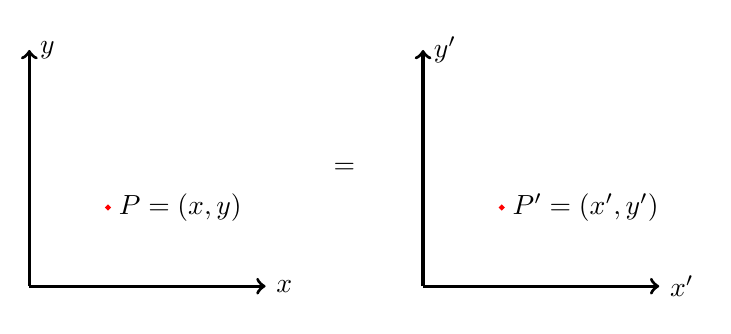
\begin{tikzpicture}
		\draw[very thick, black, ->] (0,0) -- (3,0) node[right] {$x$};
		\draw[very thick, black, ->] (0,0) -- (0,3) node[right] {$y$};
		\draw[very thick, red] (1,1) circle (.1mm) node[black,right] {$P = (x,y)$};
		\node[black] at (4,1.5) {$=$};
		\draw[very thick, black, ->] (5,0) -- (8,0) node[right] {$x'$};
		\draw[very thick, black, ->] (5,0) -- (5,3) node[right] {$y'$};
		\draw[very thick, red] (6,1) circle (.1mm) node[black,right] {$P' = (x',y')$};
	\end{tikzpicture}
\end{figure}

Det til trods havde flere af fysikere i slutningen af 1800-tallet og begyndelsen af 1900-tallet en forestilling om at der fandtes et absolutsystem, som kunne favoriseres frem for alle andre initialsystemer. Til dette system var knyttet et hypotetisk medium kaldet ``\emph{�teren}''\index{�teren}, tanken var at �teren fyldte hele universet, og at lys kunne udbrede sig i �teren p� samme vis som lydb�lger udbredes i luft.